% ME 299 project report, Om Mohan Pawar (25110218), IIT Gandhinagar. IEEE conference format, 5 pages.
% Build: latexmk -pdf main.tex   (copy main.pdf to ../docs/report.pdf)
% Figures in figs/ are drawn from the RA-L/ results and the CAD at their printed size.
\documentclass[conference]{IEEEtran}
\IEEEoverridecommandlockouts
\usepackage[T1]{fontenc}
\usepackage{newtxtext,newtxmath}
\usepackage{amsmath,bm}
\usepackage{graphicx,booktabs,array}
\usepackage{xcolor}
\usepackage[hidelinks]{hyperref}
\usepackage{cite}
\newtheorem{proposition}{Proposition}

\newcommand{\DRD}{D_{\mathrm{RD}}}
\newcommand{\dl}{\delta\bm{\ell}}
\newcommand{\lam}{\bm{\lambda}}
\newcommand{\R}{\mathbb{R}}
\newcommand{\Exp}{\operatorname{Exp}}
\setlength{\abovedisplayskip}{3pt}\setlength{\belowdisplayskip}{3pt}
\setlength{\abovedisplayshortskip}{1pt}\setlength{\belowdisplayshortskip}{2pt}
\setlength{\textfloatsep}{7pt plus 2pt minus 2pt}
\setlength{\dbltextfloatsep}{7pt plus 2pt minus 2pt}
\setlength{\floatsep}{5pt plus 2pt minus 2pt}
\renewcommand{\topfraction}{0.92}\renewcommand{\dbltopfraction}{0.92}\renewcommand{\textfraction}{0.06}
\setcounter{topnumber}{3}\setcounter{dbltopnumber}{2}
\pdfinfo{/Title (From Geometry to a Real-Time Digital Twin of Rolling-Disc Notched Tendon-Driven Continuum Robots) /Author (Om Mohan Pawar)}

\begin{document}

\title{From Geometry to a Real-Time Digital Twin of Rolling-Disc Notched Tendon-Driven Continuum Robots%
\thanks{ME 299 project report, IIT Gandhinagar, November 2026. Code, data and results:
\protect\url{https://github.com/om-mpawar/ME299-25110218}.}}

\author{\IEEEauthorblockN{Om Mohan Pawar (25110218)}
\IEEEauthorblockA{Department of Mechanical Engineering\\ Indian Institute of Technology Gandhinagar}
\and
\IEEEauthorblockN{Supervisor: Prof.\ Madhu Vadali}
\IEEEauthorblockA{IITGN Robotics Laboratory\\ Indian Institute of Technology Gandhinagar}}

\maketitle

\begin{abstract}
Printed rolling-disc notched tubes are cheap tendon-driven continuum robots, but there is no rule for choosing their
notches and no live model of their shape that needs no sensor. This report covers both. Part~A, submitted to ICRA 2027,
maps the notch geometry to bend, stroke and force with an automated CAD-to-FEM pipeline (616 simulations) and three
prototypes: the disc diameter sets curvature, the length sets reach, and 42 to 47\,\% of the tendon stroke is axial
compression. Part~B, in preparation for IEEE RA-L, is a digital twin that predicts the whole backbone from the servo
displacements alone. The module is a beam whose cross-sections come from the CAD; the tendon map is exactly linear and
symmetric positive definite, so pull-only tensions solve a strictly convex program, and gravity enters by a fixed
point. Instead of learning the shape, we identify the module's compliance law through the exact solver on one and two
modules. Unchanged, it predicts four modules (640\,mm) to 0.50\,mm of FEM, 0.08\,\% of length, in 1 to 4\,ms per pose,
where constant curvature errs by 121\,mm and a physics-informed network must be retrained.
\end{abstract}

\begin{IEEEkeywords}
Continuum robots, tendon-driven, digital twin, finite element method, system identification, scientific machine learning.
\end{IEEEkeywords}

% =====================================================================================================================
\section{Introduction}
A tendon-driven continuum robot (TDCR) bends along its whole body when tendons in its wall are pulled, which suits
confined spaces~\cite{webster2010,burgnerkahrs2015}. Ours is a printed TPU tube with two orthogonal families of
rolling-disc notches (Fig.~\ref{fig:robot}); 160\,mm modules stack, and distal tendons run through proximal modules. Two
questions drive the work. \emph{Design:} which geometry gives a wanted bend, and what stroke and force
does it cost? \emph{Model:} can the whole shape of a stack be predicted in real time from the servo commands, with no
sensor on the robot, for any number of modules? The contributions are:
\begin{enumerate}
\item SWEEP, an unattended CAD-to-FEM pipeline, and a 616-run study of how notch geometry sets curvature, reach,
stroke and tension (Section~\ref{sec:a}; ICRA 2027, second author).
\item A twin built from the CAD's sections with an exact, convex pull-only solver and gravity (Section~\ref{sec:model}).
\item Identification of the module's law, not its shape, through that solver, and its transfer from one and two
modules to four (Sections~\ref{sec:ident}, \ref{sec:results}).
\end{enumerate}

\begin{figure}[t]
\centering
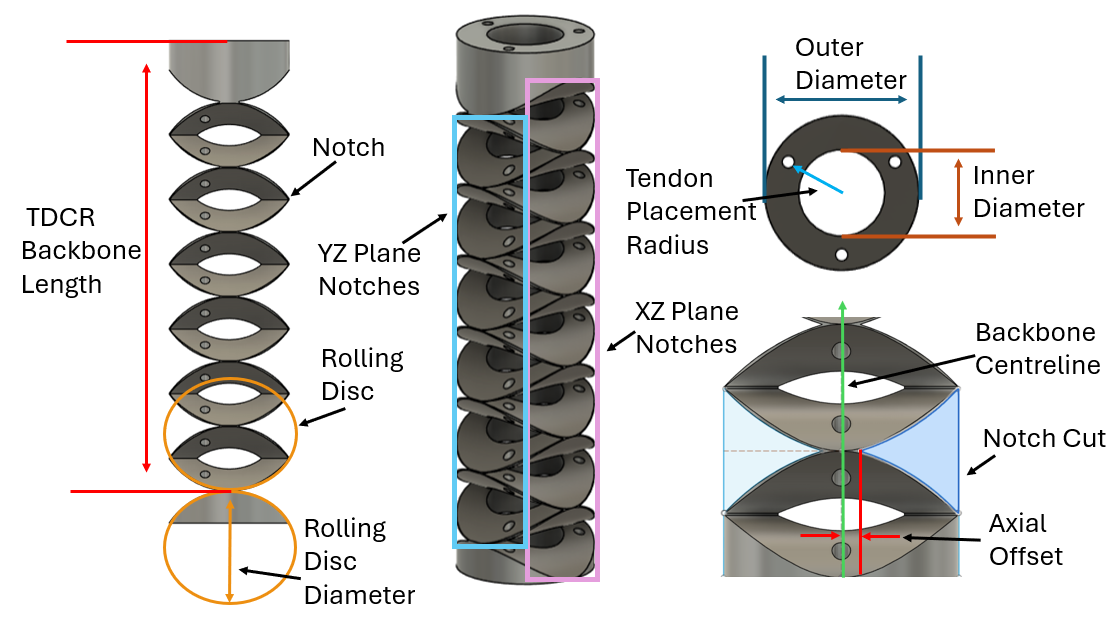
\includegraphics[height=32mm]{figs/design_params.png}\hfill
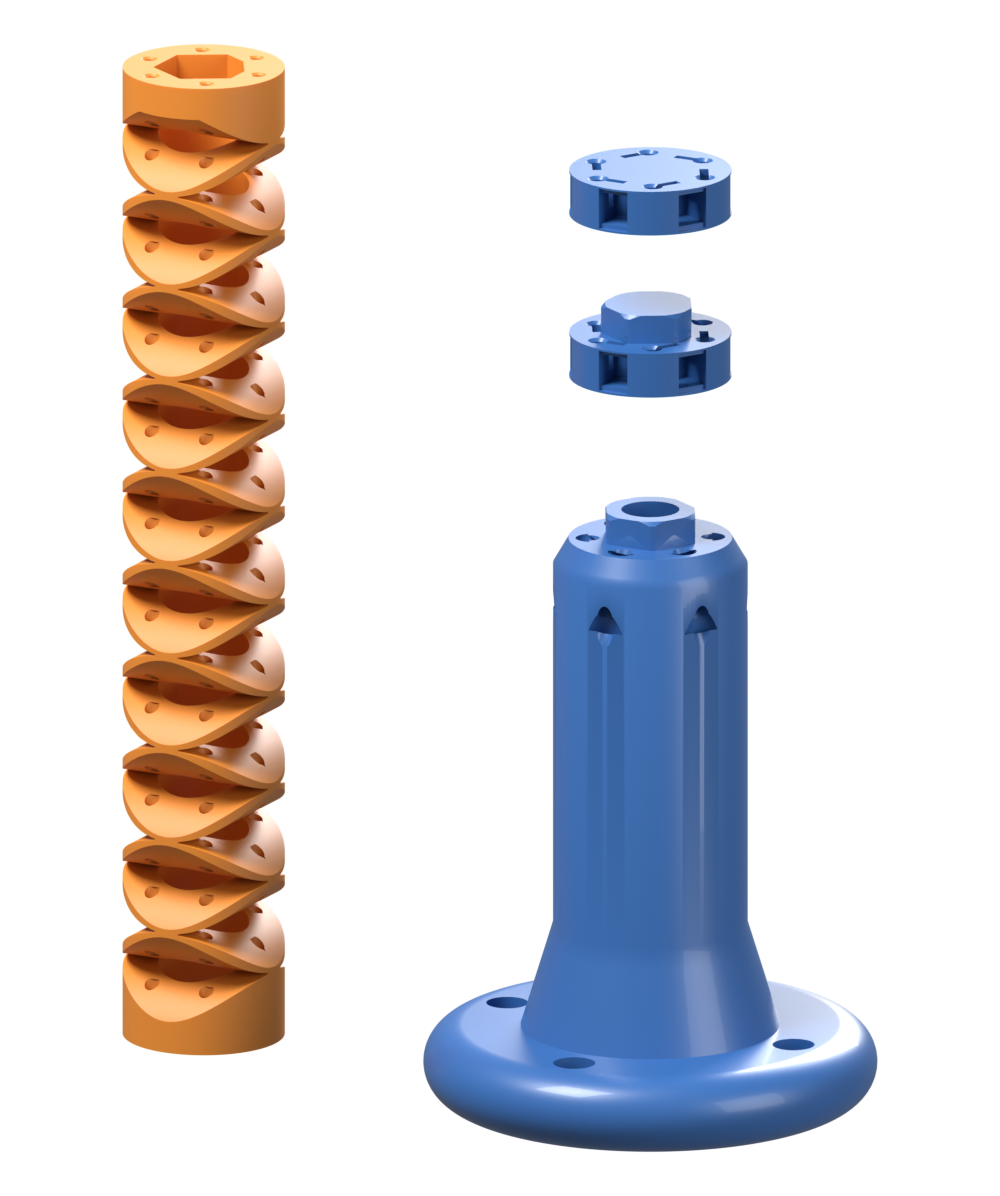
\includegraphics[height=32mm]{figs/hw_parts_render.png}
\caption{The module and its design parameters (left): disc diameter $\DRD$, length $L$, outer and inner diameters
$D_o, D_i$, tendon radius, notch offset. Right: parts designed for the four-module build (TPU module, PLA couplers,
base column).}
\label{fig:robot}
\end{figure}

\begin{figure*}[t]
\centering
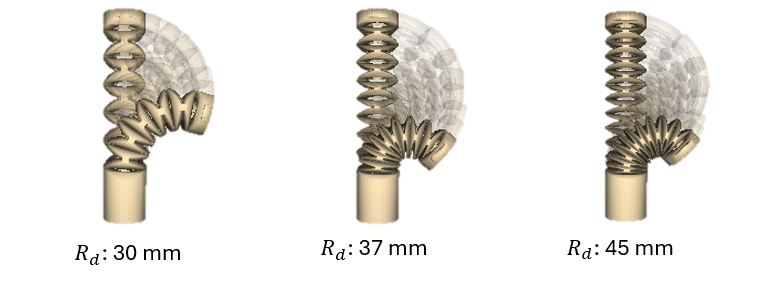
\includegraphics[height=34mm]{figs/sofa_renders.png}\hfill
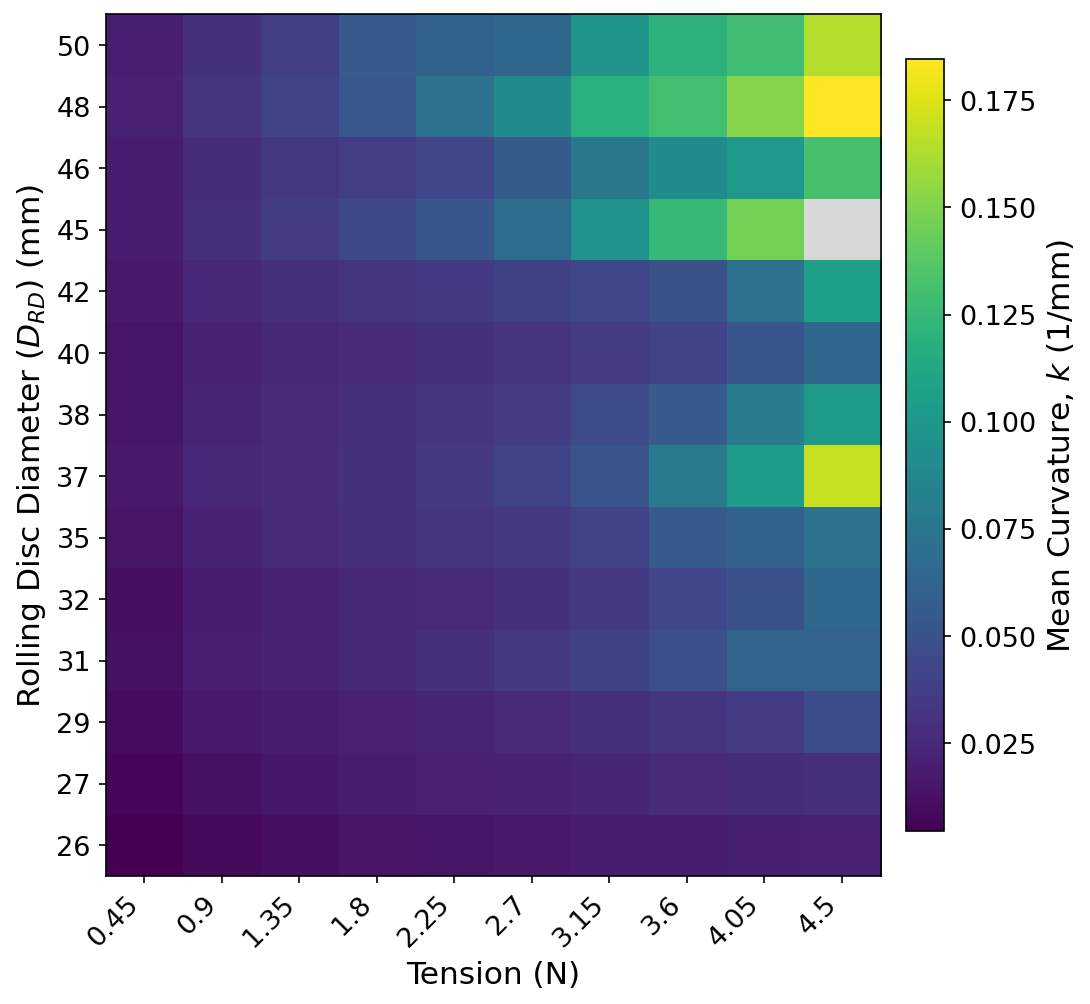
\includegraphics[height=34mm]{figs/heat_drd_curv.png}\hfill
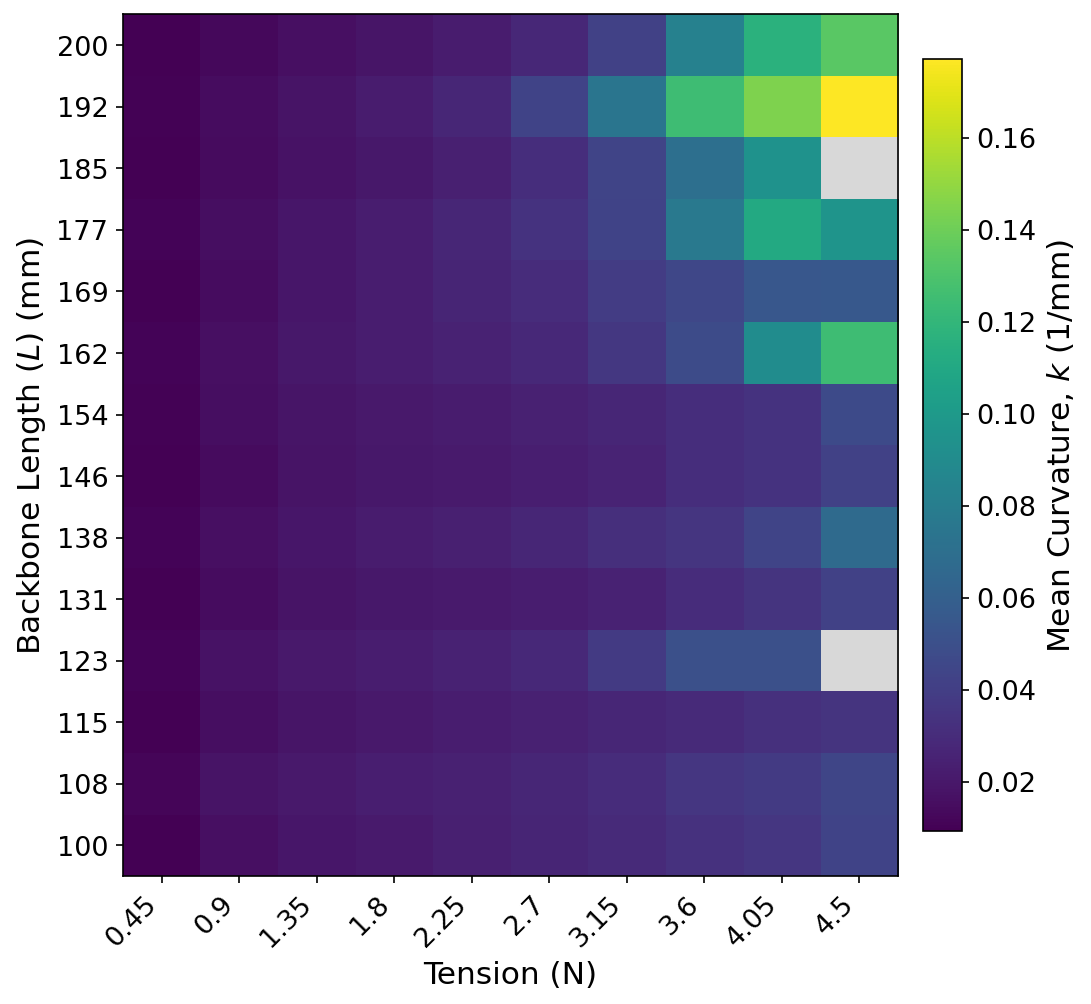
\includegraphics[height=34mm]{figs/heat_L_curv.png}
\caption{Part A. Left: the same load on three disc diameters ($R_d$ in the labels is $\DRD$); a larger disc packs more
notches and bends further. Middle and right: mean curvature $\bar\kappa$ (1/mm) against tension for the disc-diameter
and length sweeps; grey cells did not settle. The claims use $T\le0.9$\,N.}
\label{fig:sweep}
\end{figure*}

\section{Related Work}
Constant-curvature (CC) kinematics treat each section as an arc~\cite{webster2010}. Camarillo et al.\ model tendon loads as a moment and an axial
force on every section passed, with coupled routing and slack as a complementarity problem~\cite{camarillo2008,
camarillo2009}; I derived the same pull-only model before finding it, verified the two agree to $3\times10^{-6}$, and
moved the contribution to identification and transfer. Cosserat rods give the same physics by shooting~\cite{rucker2011,oliverbutler2019}; SOFA with SoftRobots is our FEM
ground truth~\cite{faure2012,coevoet2017,duriez2013}. Shape estimation uses sensors or learned
residuals~\cite{lilge2022,feliutalegon2025}, and physics-informed networks (PINNs) learn one robot's
solution~\cite{feizi2026,danesh2026,zhan2025}. The closest work calibrates pneumatic modules one at a time~\cite{kim2025};
with tendons every module is loaded by those above it, so none can be calibrated alone. Errors are in \% of
length~\cite{rao2020}.

% =====================================================================================================================
\section{Part A: How Geometry Governs Compliance}\label{sec:a}
\begin{figure}[t]
\centering
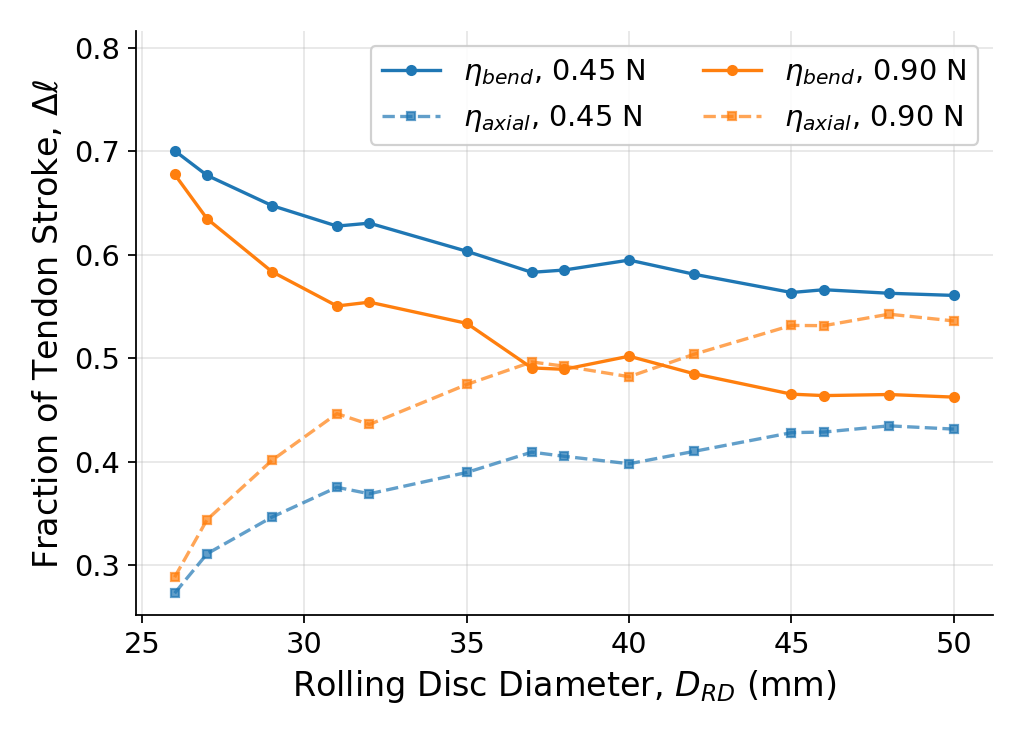
\includegraphics[width=0.495\columnwidth]{figs/stroke_D.png}\hfill
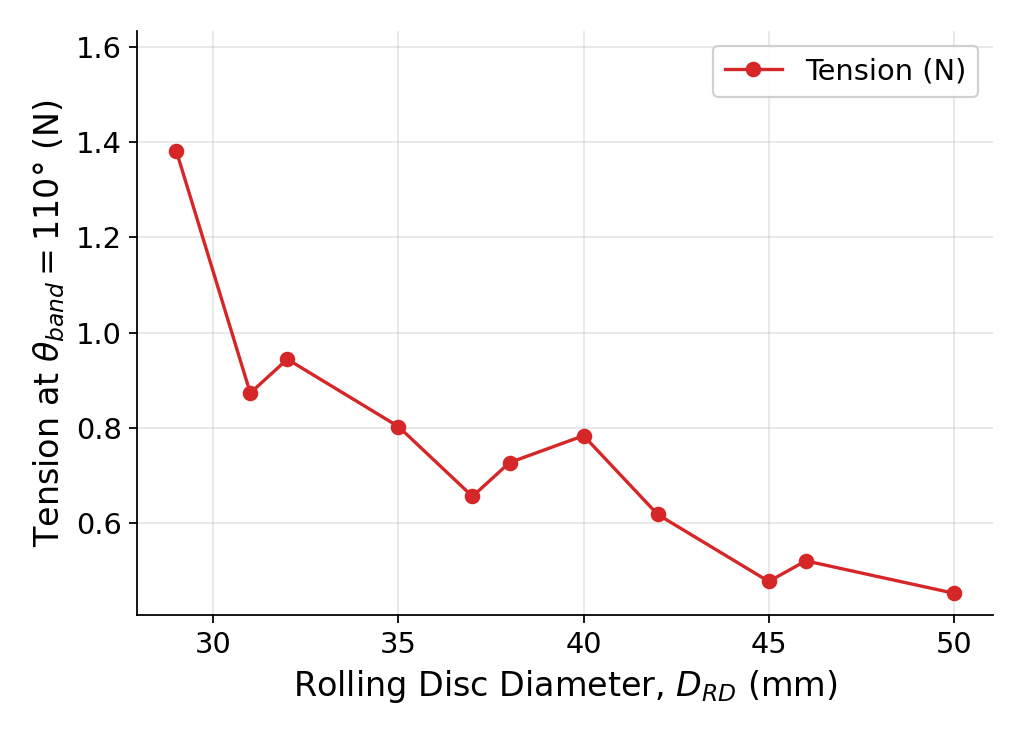
\includegraphics[width=0.495\columnwidth]{figs/tension_D.png}
\caption{Stroke budget~\eqref{eq:budget} against $\DRD$. Left: bending and axial fractions at 0.45 and 0.9\,N. Right:
tension for a $110^\circ$ bend.}
\label{fig:stroke}
\end{figure}
\begin{figure}[t]
\centering
\begin{minipage}[c]{0.5\columnwidth}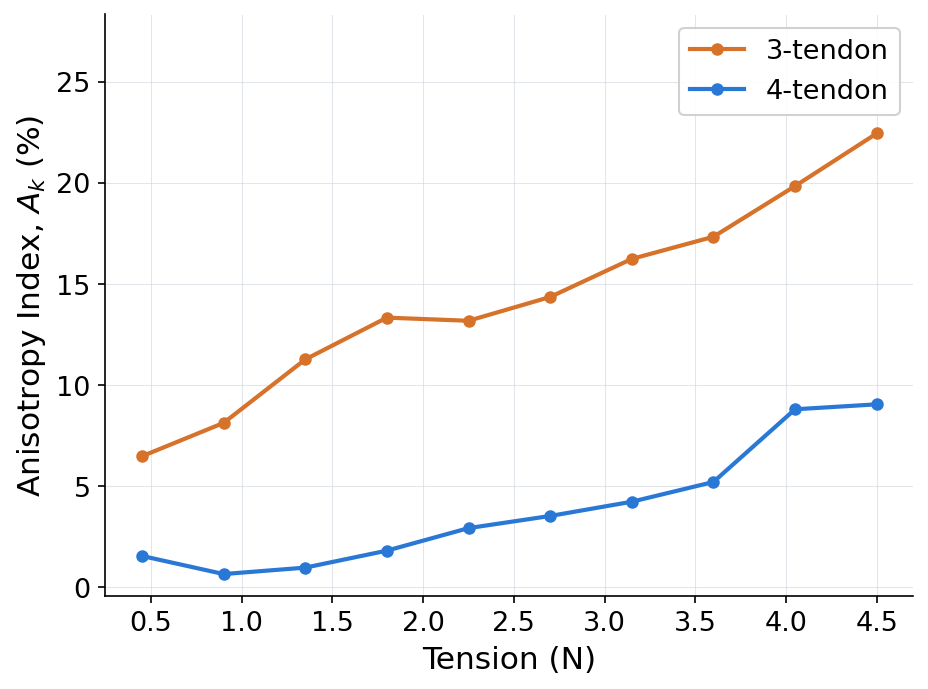
\includegraphics[width=\linewidth]{figs/aniso_27.png}\end{minipage}\hfill
\begin{minipage}[c]{0.47\columnwidth}\centering\footnotesize\setlength{\tabcolsep}{2.5pt}
\begin{tabular}{@{}cccc@{}}
\toprule
$\DRD$ & centre- & tip & axial\\
(mm) & line & & \\
\midrule
30 & 18.5 & 20.9 & 43.1\\
67.89 & 10.1 & 23.5 & 11.9\\
86.84 & 16.3 & 64.7 & 23.9\\
\bottomrule
\end{tabular}\end{minipage}
\caption{Left: anisotropy $A_\kappa$ against tension, three and four tendons ($\DRD=27$\,mm). Right: three printed
prototypes against simulation, NRMSE in \% of length.}
\label{fig:aniso}\label{tab:proto}
\end{figure}
\subsection{Parametric backbone}
A notch is cut from a tube of outer radius $R_o$ by two discs of radius $R_d=\DRD/2$ whose centres are $\DRD$ apart, so
its height and the nominal pitch with a clearance $c$ are
\begin{equation}
h = \DRD - 2\sqrt{R_d^2-R_o^2},\qquad p_0 = h + c .
\label{eq:notch}
\end{equation}
On a notched length $L$ with a top margin $m_t$, the number of notches and the pitch they are spread to are
\begin{equation}
N_n = \Big\lfloor \frac{L-m_t-h}{p_0}\Big\rfloor + 1,\qquad p=\frac{L-m_t-h}{N_n-1},
\label{eq:count}
\end{equation}
which for $\DRD=30$\,mm and $L=150$\,mm gives $h=13.4$\,mm, ten notches and $p=14.79$\,mm, as in the CAD. The disc
diameter therefore sets how many notches fit. Two families at $90^\circ$ alternate along the tube; each notch leaves two
bridges of half-width $e$.


\begin{figure*}[t]
\centering
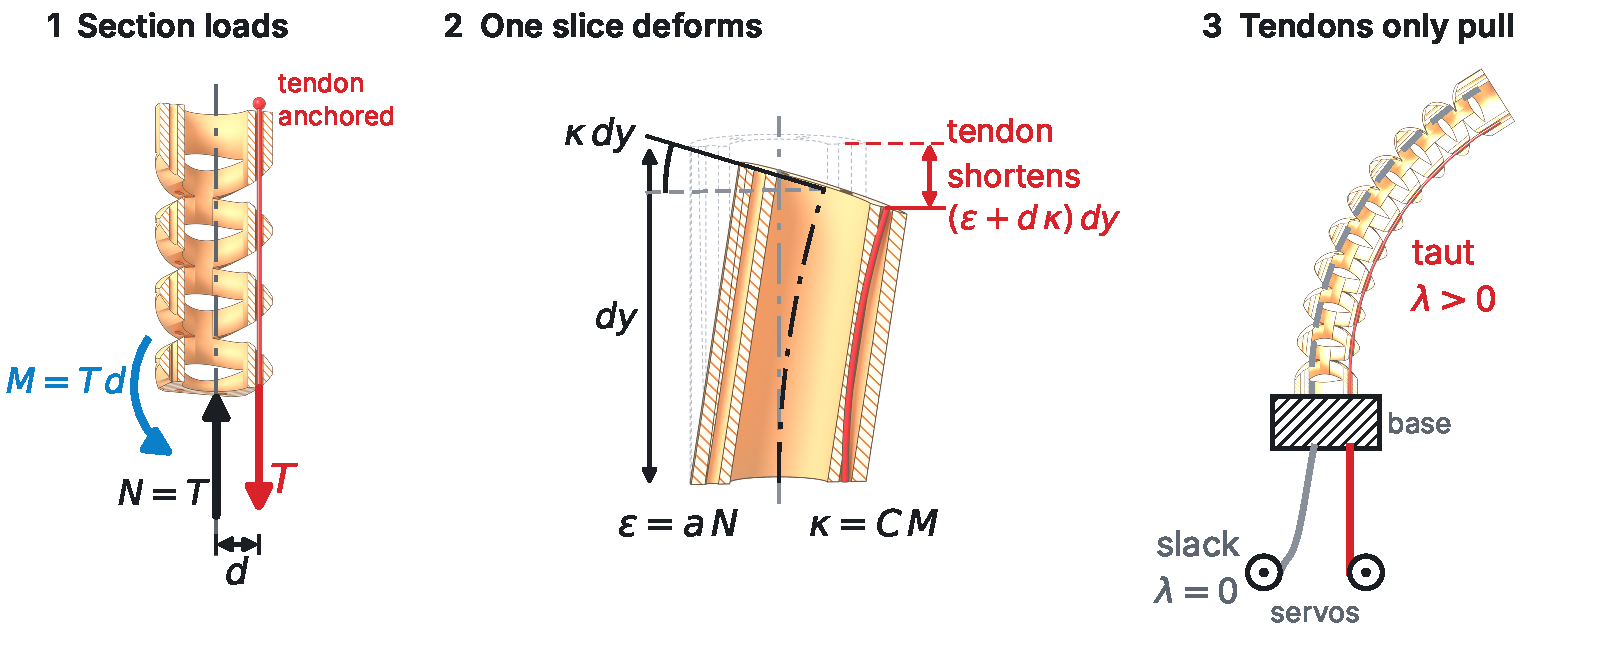
\includegraphics[width=0.74\textwidth]{figs/physics_r.pdf}
\caption{The physics, drawn on half sections of the CAD. (1) A tendon of tension $T$ at offset $d$ loads every section it
passes with $N=T$ and $M=Td$. (2) A slice of height $dy$ shortens by $\varepsilon\,dy$ and bends by $\kappa\,dy$; the
tendon's path shortens by $(\varepsilon+d\kappa)\,dy$ (exaggerated). (3) The module bent by the twin: the pulled tendon
is taut, the paid-out one slack.}
\label{fig:physics}
\end{figure*}

\subsection{Pipeline and metrics}
SWEEP builds each design in CadQuery with one Boolean cut, meshes it with CGAL tetrahedra and pulls one tendon at a time
through a load sequence in SOFA, logging the centreline $\{\bm p_i\}$ once the tip has settled. My part was the port to
SOFA 25.06, parallel and staged sweeps, a mesh-volume check against the CAD, and per-run settling and self-contact
checks. With $\bm a=\bm p_i-\bm p_{i-1}$, $\bm b=\bm p_{i+1}-\bm p_i$ and $\bm c=\bm p_{i+1}-\bm p_{i-1}$, the
pointwise (Menger) curvature and its mean are
\begin{equation}
\kappa_i=\frac{2\,\lVert\bm a\times\bm b\rVert}{\lVert\bm a\rVert\,\lVert\bm b\rVert\,\lVert\bm c\rVert},
\qquad \bar\kappa=\frac{1}{n}\sum_i\kappa_i .
\end{equation}
The departure from a circular arc is the RMS radial residual to the best-fit (Kåsa) circle $(\bm o,\rho)$, normalised by
the arc length $\ell$; the anisotropy is the spread of $\bar\kappa$ over the tendon directions $j$ at one load:
\begin{equation}
e_{\mathrm{CC}}=\frac1\ell\Big(\frac1n\sum_i\big(\lVert\bm p_i-\bm o\rVert-\rho\big)^2\Big)^{\!1/2},\qquad
A_\kappa=\frac{\operatorname{std}_j\bar\kappa_j}{\operatorname{mean}_j\bar\kappa_j}.
\end{equation}
A tendon at offset $d$ that turns the tip by $\Theta$ and shortens the body by $\Delta L$ needs the stroke
\begin{equation}
\Delta\ell=\Theta d+\Delta L,\qquad \eta_b=\frac{\Theta d}{\Delta\ell},\quad \eta_a=\frac{\Delta L}{\Delta\ell}.
\label{eq:budget}
\end{equation}


\subsection{Results}
The study ran 14 designs $\times$ 4 tendons $\times$ 11 loads (616 runs, 614 completed), $E=56$\,MPa (measured), with
gravity. Above 0.9\,N runs stop settling or self-contact, so claims hold for $T\le0.9$\,N. Raising
$\DRD$ from 26 to 50\,mm raises the notch count from 4 to 12 and the bend at 0.9\,N from $54^\circ$ to $143^\circ$, and
$e_{\mathrm{CC}}$ about five-fold (Fig.~\ref{fig:sweep}). Doubling $L$ from 100 to 200\,mm doubles the tip travel, 78 to
157\,mm, with $\bar\kappa$ changing by under 20\,\%. The budget~\eqref{eq:budget} closes to $\eta_b+\eta_a=0.99$ on
notched designs (0.72 on a plain tube), and 42 to 47\,\% of the stroke is compression (Fig.~\ref{fig:stroke}); a larger
disc lowers the tension for $110^\circ$ from 0.87 to 0.45\,N. Four tendons suit the two notch planes: $A_\kappa$ falls
from 6.2 to 2.6\,\% in 13 of 14 designs (Fig.~\ref{fig:aniso}), with two motors driving antagonistic pairs. Three
prototypes loaded with weights agree with simulation in shape to 10 to 19\,\% of length (Fig.~\ref{fig:aniso}); the tip
agrees less well, as friction and self-contact are not modelled.


% =====================================================================================================================
\section{Part B: The Physics of the Twin}\label{sec:model}
\emph{Problem.} The module is the SWEEP design with $\DRD=30$\,mm, $L=150$\,mm, $D_o/D_i=25/14$\,mm, and three tendons
in channels at radius 9.5\,mm (sections 1--2 at $0/120/240^\circ$, 3--4 at $60/180/300^\circ$). Given the servo
displacements $\dl\in\R^{3N}$ and gravity, predict the backbone's frames every 5\,mm with no sensor on the robot.


\subsection{Section properties}
Let $z$ be the material coordinate along the backbone. From the CAD we compute, every 0.02\,mm and with the channels
removed, the area $A(z)$ and second moments $J_x=\int x^2dA$, $J_y=\int y^2dA$ (Fig.~\ref{fig:sections}). The backbone is divided into cells $c$ of
$\Delta=0.5$\,mm with compliances
\begin{equation}
\begin{aligned}
a_c&=\int_c\frac{dz}{EA},\qquad C_c=\int_c\operatorname{diag}\Big(\frac{1}{EJ_x},\frac{1}{EJ_y}\Big)dz,\\
t_c&=\int_c\frac{2(1+\nu)}{E\,(J_x+J_y)}\,dz,
\end{aligned}
\label{eq:cells}
\end{equation}
for compression, bending and twist ($E=56$\,MPa, $\nu=0.48$).

\begin{figure}[t]
\centering
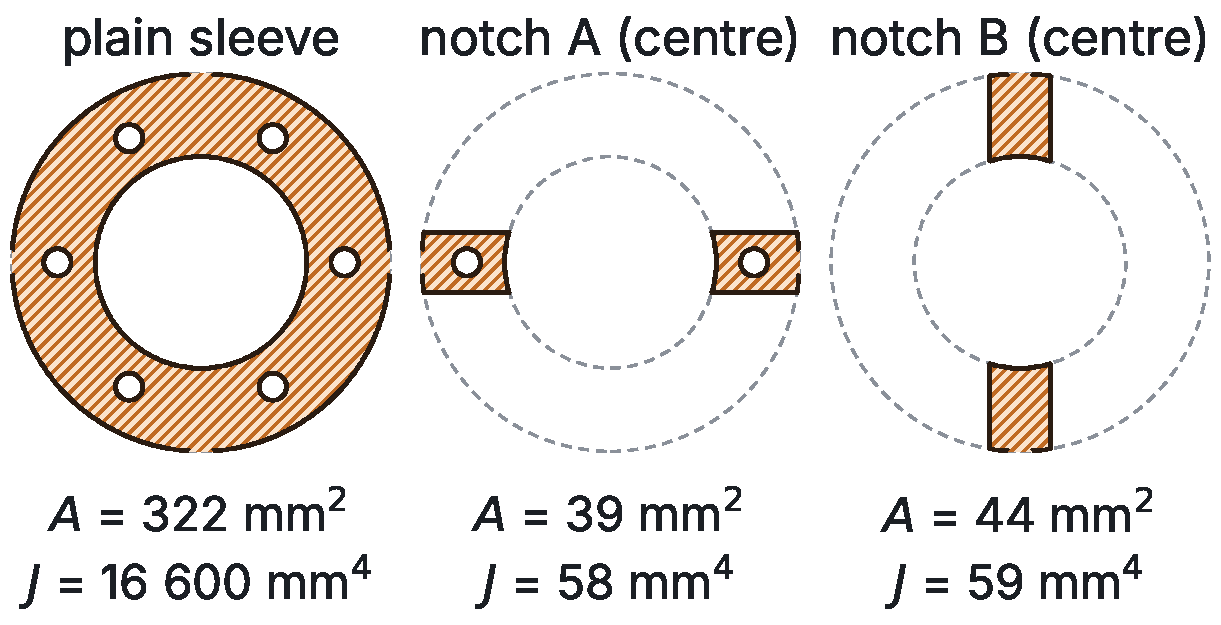
\includegraphics[width=0.9\columnwidth]{figs/sections_r.pdf}
\caption{Cross-sections of the module from the CAD (hatched: material), with the tendon channels removed. A notch keeps
two 4\,mm bridges: $A$ falls 8-fold and $\min(J_x,J_y)$ 280-fold.}
\label{fig:sections}
\end{figure}

\subsection{Tendon loads and the tendon map}
Tendon $i$, at offset $\bm d_i\in\R^2$ in the cross-section with tension $\lambda_i$, applies an axial force $\lambda_i$
and a moment $\lambda_i\bm d_i$ to every section it passes~\cite{camarillo2008,rucker2011} (Fig.~\ref{fig:physics}).
With $\tau_{ic}=1$ if tendon $i$ passes cell $c$, the cell's axial force, moment and strains are
\begin{equation}
\begin{aligned}
N_c&=\textstyle\sum_i\tau_{ic}\lambda_i, &\bm m_c&=\textstyle\sum_i\tau_{ic}\lambda_i\bm d_i,\\
\varepsilon_c&=a_cN_c, &\bm\kappa_c&=C_c\bm m_c,
\end{aligned}
\label{eq:strain}
\end{equation}
where $\bm\kappa_c$ is the integrated curvature towards $x$ and $y$. Tendon $i$'s path shortens by
$\sum_c\tau_{ic}(\varepsilon_c+\bm d_i^\top\bm\kappa_c)$, and the servo also takes up its stretch $c_tL_i\lambda_i$.
Since the channels are straight in the material frame, this is linear at any bend:
\begin{equation}
\dl=G\lam,\qquad G_{ij}=\sum_c\tau_{ic}\tau_{jc}\big(a_c+\bm d_i^\top C_c\bm d_j\big)+c_tL_i\,\delta_{ij}.
\label{eq:G}
\end{equation}

\begin{proposition}\label{prop:spd}
$G$ is symmetric positive definite, and $\frac12\lam^\top G\lam$ is the complementary energy of the backbone and tendons.
\end{proposition}
\begin{IEEEproof}
Symmetry is evident from~\eqref{eq:G}. Substituting~\eqref{eq:strain},
\begin{equation}
\tfrac12\lam^\top G\lam=\tfrac12\sum_c\big(a_cN_c^2+\bm m_c^\top C_c\bm m_c\big)+\tfrac12\sum_i c_tL_i\lambda_i^2 .
\label{eq:energy}
\end{equation}
It vanishes only if $N_c=0$ and $\bm m_c=\bm 0$ in every cell. In the top module only its own three tendons act, and
the vectors $(1,\bm d_i)$ of three channels $120^\circ$ apart are linearly independent, so their tensions are zero;
peeling modules from the tip gives $\lam=\bm 0$.
\end{IEEEproof}

\subsection{Pull-only tensions}
A tendon cannot push. With slack $w_i=(G\lam-\dl)_i$, the tensions satisfy the linear complementarity problem
$\lam\ge\bm0$, $\bm w\ge\bm0$, $\lam^\top\bm w=0$, which is exactly the KKT system of
\begin{equation}
\lam^\star=\arg\min_{\lam\ge\bm0}\ \tfrac12\,\lam^\top G\lam-\dl^\top\lam .
\label{eq:qp}
\end{equation}
By Proposition~\ref{prop:spd} it is strictly convex with a unique solution: minimum complementary energy minus the work
of the prescribed displacements. With $G=LL^\top$ the objective is $\frac12\lVert L^\top\lam-L^{-1}\dl\rVert^2$ up to a
constant, so we solve it exactly by non-negative least squares on the Cholesky factor. Slack tendons and the coupling of distal tendons through proximal modules~\cite{camarillo2009} follow
from the same $G$.

\begin{figure*}[t]
\centering
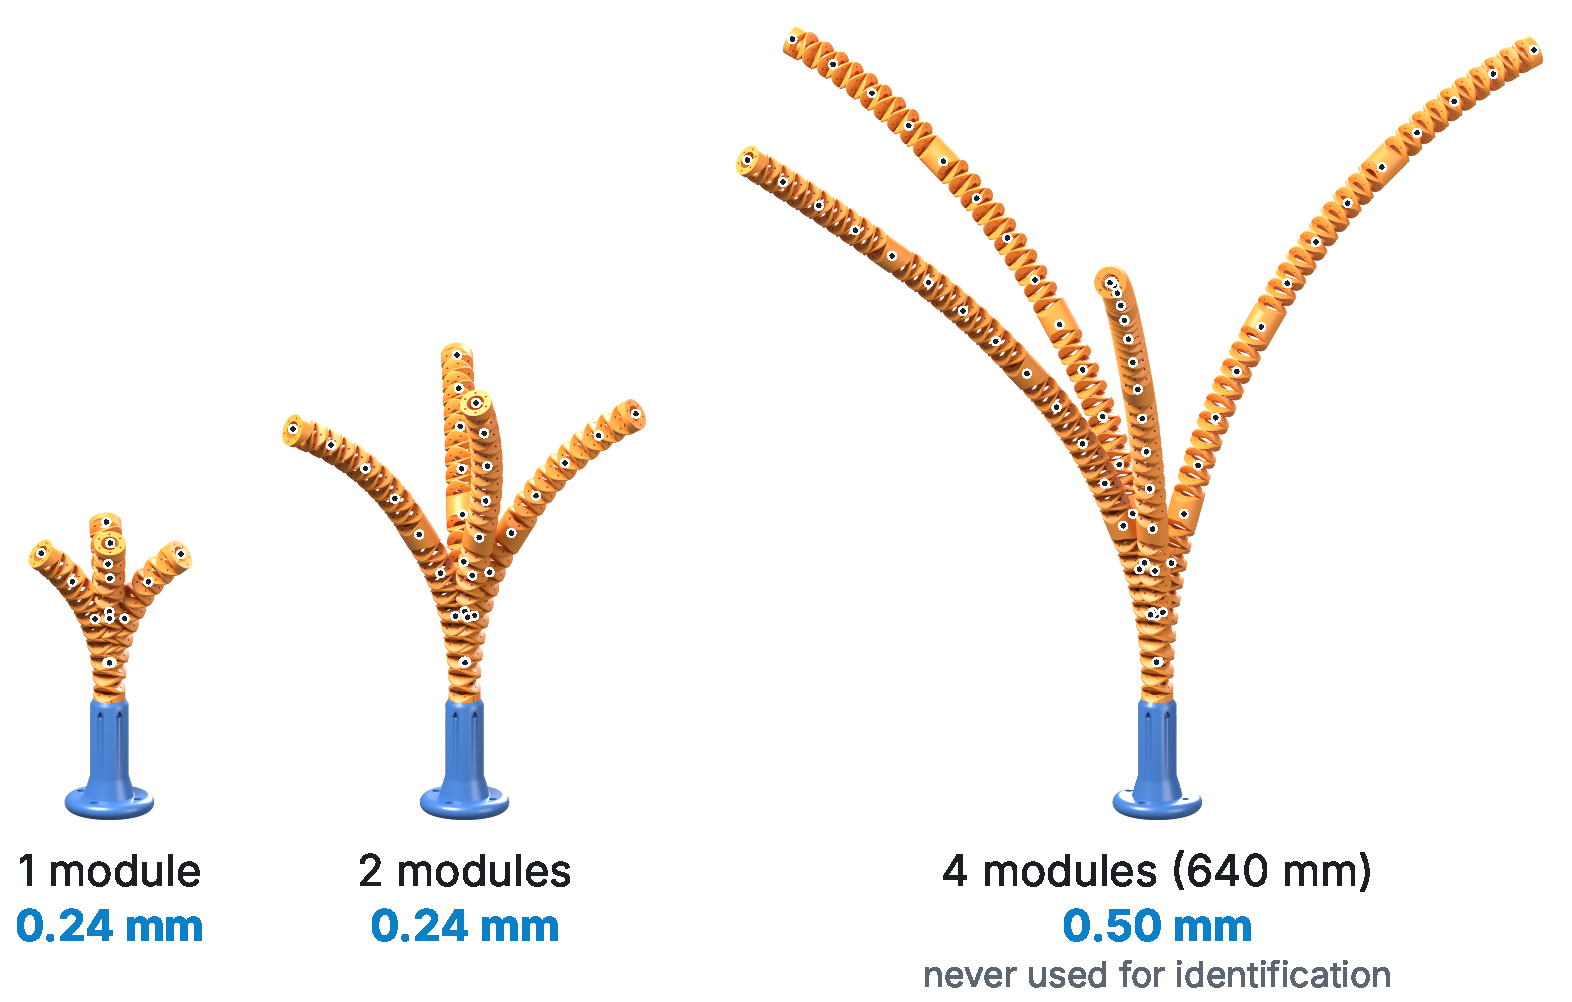
\includegraphics[width=0.565\textwidth]{figs/shapes_r.pdf}\hfill
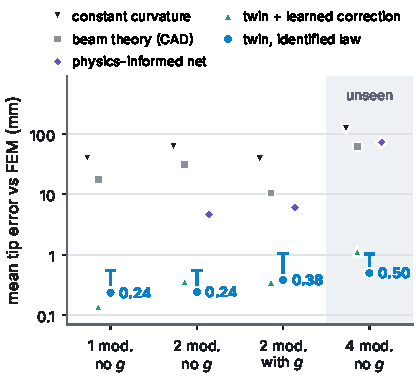
\includegraphics[width=0.415\textwidth]{figs/transfer_r.pdf}
\caption{Transfer to configurations never used for identification. Left: the twin rendered on the CAD for the four most
bent held-out poses of 1, 2 and 4 modules, at one scale; dots are the FEM centreline. Right: mean tip error against FEM,
bars to the 95th percentile; 60 to 100 held-out poses per set, tip bends up to $75^\circ$.}
\label{fig:results}
\end{figure*}

\subsection{Kinematics}
Each cell turns by the rotation vector $\bm\omega_c=(-\kappa_{c,y},\,\kappa_{c,x},\,\phi_c)$ in its own frame, $\phi_c$
being the twist. Frames and positions follow by the midpoint rule,
\begin{equation}
\begin{aligned}
R_{c+1}&=R_c\Exp(\bm\omega_c),\\
\bm p_{c+1}&=\bm p_c+R_c\Exp(\tfrac12\bm\omega_c)\,(\Delta-\varepsilon_c)\,\bm e_z,
\end{aligned}
\label{eq:kin}
\end{equation}
and each joint adds a rigid straight segment. Without gravity $E$ cancels: scaling $G$ scales $\lam$ inversely.

\subsection{Gravity}
Module mass is spread over the cells in proportion to the CAD area, $m_c$, with weight $\bm F_c=m_c\bm g$. From the
current shape, the weight distal to cell $c$ gives, in the cell frame,
\begin{equation}
\bm n_c=R_c^\top\!\!\sum_{c'>c}\!\bm F_{c'},\qquad
\bm\mu_c=R_c^\top\!\!\sum_{c'>c}\!(\bm p_{c'}-\bm p_c)\times\bm F_{c'},
\end{equation}
which adds the strains $\bm\kappa^g_c=C_cS\bm\mu_c$, $\varepsilon^g_c=-a_cn_{c,z}$ and the twist $\phi_c=k_T\,t_c\,\mu_{c,z}$,
with $S$ picking the bending components and $k_T$ the torsion factor of Section~\ref{sec:ident}. The weight also shortens
the tendon paths by $h_i=\sum_c\tau_{ic}(\varepsilon^g_c+\bm d_i^\top\bm\kappa^g_c)$, so the tensions are re-solved
from~\eqref{eq:qp} with $\dl-\bm h$. Writing $\bm x$ for all gravity strains and $\Phi$ for one pass of shape, loads,
tensions and strains, the twin iterates
\begin{equation}
\bm x^{k+1}=(1-\beta_k)\,\bm x^k+\beta_k\,\Phi(\bm x^k),
\label{eq:fp}
\end{equation}
halving $\beta_k$ (from 0.5, down to 0.05) whenever the update grows, until the change is below $10^{-4}$ per cell. It
is warm-started from the previous call, so following the servos takes a few iterations.

% =====================================================================================================================
\section{Part B: Identifying the Module Law}\label{sec:ident}
\subsection{Learn the law, not the solution}
Plane sections miss how a short notch deforms (the discs compress like wave springs). Rather than learn shapes, we
correct the law~\eqref{eq:cells} and keep the exact solver:
\begin{equation}
a_c(\bm\theta)=a_c^{\mathrm{CAD}}\exp\!\big(s_a\chi_c+\bm b(z_c)^\top\bm f_a\big),
\label{eq:law}
\end{equation}
and likewise for each bending direction, where $\chi_c=1$ in cells a notch cuts, $s$ is one log-scale per compliance and
$\bm b$ a linear spline basis along the module (17 knots). Positive factors keep $G$ positive definite, so the fitted
model is still convex and composes to any $N$. The parameters $\bm\theta=(\bm s,\bm f)$ are fitted through the full
model to SOFA poses of one and two modules,
\begin{equation}
\begin{aligned}
\min_{\bm\theta}\ &\sum_{\text{sets }q}\frac{1}{P_qK_q}\sum_{p,k}\big\lVert\bm p_k(\bm\theta;\dl_p,\bm g_q)-\bm p^{\mathrm{FEM}}_{pk}\big\rVert^2\\
&+\rho\lVert\bm f\rVert^2+\sigma\lVert D\bm f\rVert^2,
\end{aligned}
\label{eq:fit}
\end{equation}
over $P_q$ poses and $K_q$ stations per set, with $D$ the first difference ($\rho=0.02$, $\sigma=0.5$), by
trust-region least squares with a finite-difference Jacobian. On 675 poses (Fig.~\ref{fig:law}) the notched cells come
out $\times20.2$ softer axially and $\times5.9$, $\times5.3$ in bending; the profile stays within 13\,\% of constant. A
SOFA twist test of one module gives the torsion factor $k_T=2.45$.

\begin{figure}[t]
\centering
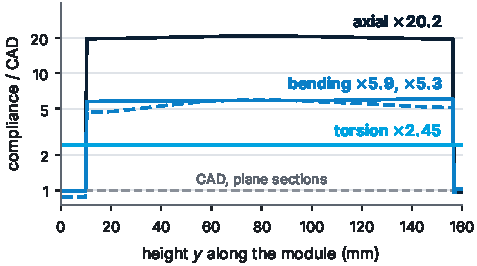
\includegraphics[width=\columnwidth]{figs/law_r.pdf}
\caption{The identified law~\eqref{eq:law}: each compliance of one module divided by its plane-section value. Four
scales carry it; the plain sleeve keeps the CAD value.}
\label{fig:law}
\end{figure}

\subsection{What the data can identify}
\begin{proposition}\label{prop:mass}
Scaling every compliance ($a_c$, $C_c$, $t_c$, $c_t$) by $k>0$ and every mass by $1/k$ leaves the shape unchanged for
every $\dl$ and $\bm g$.
\end{proposition}
\begin{IEEEproof}
$G\to kG$ gives $\lam\to\lam/k$, so~\eqref{eq:strain} is unchanged; the gravity strains are compliance times weight,
also unchanged; hence~\eqref{eq:fp} has the same fixed point.
\end{IEEEproof}
Shape data cannot separate softness from weight, so on hardware the modules are weighed, not fitted; without gravity the
overall scale is unobservable and a small ridge fixes it.

\begin{proposition}\label{prop:one}
For one module with all three tendons taut, rigid tendons and no gravity, the total shortening $s$ and bend
$\bm\Theta=\sum_c\bm\kappa_c$ are fixed by $\dl$ alone: $s=\frac13\sum_i\delta\ell_i$ and $\bm d_i^\top\bm\Theta=\delta\ell_i-s$.
\end{proposition}
\begin{IEEEproof}
All tendons pass every cell, so $\delta\ell_i=s+\bm d_i^\top\bm\Theta$; channels $120^\circ$ apart give
$\sum_i\bm d_i=\bm0$.
\end{IEEEproof}
Taut one-module poses therefore carry no information on the compliances. Our FEM poses each have a slack tendon, and
then one module does fix the axial-to-bending ratio (Jacobian singular values 622, 545 and 0.41, the weak direction being
the overall scale, as Proposition~\ref{prop:mass} predicts); two modules, where a distal pull divides between modules,
make it robust.

\begin{proposition}\label{prop:pre}
For $N$ identical modules, the pretension giving every tendon the same tension pulls section $s$ by
$p_s=p_1\sum_{j\le s}(N-j+1)/N$: $1:1.75:2.25:2.5$ for four modules.
\end{proposition}
\begin{IEEEproof}
With $\lam=\lambda\bm1$ the bending terms of~\eqref{eq:G} cancel in each section ($\sum_{i\in s}\bm d_i=\bm0$), and
module $j$ carries the axial force of the $3(N-j+1)$ tendons passing it.
\end{IEEEproof}

\subsection{Few-shot hardware calibration}
Five numbers are fitted on about 15 motion-capture poses of two modules: log-scales on the axial and two bending compliances, the tendon compliance $c_t$, and a moment-arm offset
$\Delta d$ (a wire bears nearer the axis than SOFA's cable), minimising
$\sum_{p,k}\lVert\bm p_k-\hat{\bm p}_k\rVert^2+\ell^2\lVert\operatorname{Log}(R_k^\top\hat R_k)\rVert^2$ with $\ell=100$\,mm.
On synthetic data with 0.3\,mm noise this recovers the bending scale to 0.003 and $\Delta d$ to 0.02\,mm, while a free
mass drifts by tens of percent (Proposition~\ref{prop:mass}).

% =====================================================================================================================
\section{Results}\label{sec:results}

Table~\ref{tab:results} and Fig.~\ref{fig:results} compare five models on held-out FEM poses. The CC baseline puts one
arc on each module, $\delta\ell_i=r\,\ell_t\sum_{m\le s(i)}\kappa_m\cos(\psi_i-\alpha_m)$, solved for $(\kappa_m,
\alpha_m)$ by least squares; ignoring compression, it over-bends 1.7-fold. A learned (GP) correction helps where trained
but doubles the error on four modules, and PINNs must be retrained for four. The identified law stays at 0.24 to
0.50\,mm in every set, including four modules (640\,mm, 0.08\,\% of length) never used for fitting; its scales alone,
fitted on two-module data, give 0.67\,mm on four. A pose takes a median of 1.0, 1.9 and 4.0\,ms for 1, 2 and 4 modules with gravity (slowest call 26\,ms, laptop
CPU), against 357\,ms for a Cosserat rod. The solver matches closed-form beam cases to under 1\,\textmu m and an
independent Cosserat rod to 0.004\,mm; 132 automated tests and one command regenerate every number. All errors are
against FEM, whose coarse and fine meshes differ by about 0.6\,mm at the tip (earlier robot), the scale of the twin's
error.

\begin{table}[t]
\caption{Mean tip error against FEM on held-out poses (mm)}
\label{tab:results}
\centering\footnotesize
\setlength{\tabcolsep}{3.2pt}
\begin{tabular}{@{}lcccc@{}}
\toprule
Modules, gravity & 1, no & 2, no & 2, yes & 4, no$^*$\\
\midrule
Constant curvature & 39.5 & 61.8 & 38.3 & 120.9\\
Beam theory from CAD & 17.8 & 30.8 & 10.5 & 61.7\\
PINN (forward) & -- & 4.6 & 6.0 & 72.5$^\dagger$\\
Twin + GP correction & 0.14 & 0.36 & 0.35 & 1.12\\
\textbf{Identified law} (mean) & \textbf{0.24} & \textbf{0.24} & \textbf{0.38} & \textbf{0.50}\\
\quad 95th percentile & 0.54 & 0.55 & 1.04 & 1.02\\
\bottomrule
\end{tabular}\\[2pt]
{\scriptsize $^*$never used for fitting. $^\dagger$retrained on four-module physics.}
\end{table}

% =====================================================================================================================
\section{Future Work: Towards Sensor-Free Cavity Insertion}\label{sec:future}
\emph{(1) Hardware validation (now):} calibrate the five numbers on 15 poses of two modules and test on four, passing if
the mean tip error is at most 2\,\% of length (13\,mm), a bar set before any data. \emph{(2) Contact in the twin:} a
wall is one-sided like a tendon; contact forces $f_k\ge0$ with gaps $g_k(\bm x)\ge0$ and $f_kg_k=0$ form a second
complementarity problem of the same kind as~\eqref{eq:qp}, solved inside~\eqref{eq:fp}, to be checked against FEM and
motion capture with a wall. \emph{(3) Cavity insertion:} feed the stack through an opening while the twin chooses the
servo commands, passing if it reaches a target inside a printed cavity. If residuals grow with bend, a convex notch energy replaces the linear law.

\section{Conclusion and Learning Outcomes}
The notch geometry gives separate control of curvature and reach, at the price of a stroke budget in which compression
takes almost half. A module law identified inside an exact, convex model of the CAD transfers from one and two modules
to four to 0.08\,\% of length in milliseconds, where constant curvature and learned solutions do not. The project taught
continuum-robot mechanics, FEM in SOFA, convex optimisation with unilateral constraints, system identification and
scientific machine learning, and a method: test simulators on simple cases (our cables could push), search the
literature before claiming novelty, fix pass criteria before taking data, and make every number reproducible.

\section*{Acknowledgment}
I thank Prof.\ Madhu Vadali for supervision, and Divij Yadav, Krishnapriya R and Shaili Gandhi, co-authors of the ICRA
submission, for SWEEP and the prototypes.

\begin{thebibliography}{99}\footnotesize\setlength{\itemsep}{0pt}
\bibitem{webster2010} R.~J. Webster and B.~A. Jones, ``Design and kinematic modeling of constant curvature continuum robots: a review,'' \emph{Int. J. Robot. Res.}, vol.~29, no.~13, pp.~1661--1683, 2010.
\bibitem{burgnerkahrs2015} J.~Burgner-Kahrs, D.~C. Rucker, and H.~Choset, ``Continuum robots for medical applications: a survey,'' \emph{IEEE Trans. Robot.}, vol.~31, no.~6, pp.~1261--1280, 2015.
\bibitem{camarillo2008} D.~B. Camarillo, C.~F. Milne, C.~R. Carlson, M.~R. Zinn, and J.~K. Salisbury, ``Mechanics modeling of tendon-driven continuum manipulators,'' \emph{IEEE Trans. Robot.}, vol.~24, no.~6, pp.~1262--1273, 2008.
\bibitem{camarillo2009} D.~B. Camarillo, C.~R. Carlson, and J.~K. Salisbury, ``Configuration tracking for continuum manipulators with coupled tendon drive,'' \emph{IEEE Trans. Robot.}, vol.~25, no.~4, pp.~798--808, 2009.
\bibitem{rucker2011} D.~C. Rucker and R.~J. Webster, ``Statics and dynamics of continuum robots with general tendon routing and external loading,'' \emph{IEEE Trans. Robot.}, vol.~27, no.~6, pp.~1033--1044, 2011.
\bibitem{oliverbutler2019} K.~Oliver-Butler, J.~Till, and C.~Rucker, ``Continuum robot stiffness under external loads and prescribed tendon displacements,'' \emph{IEEE Trans. Robot.}, vol.~35, no.~2, pp.~403--419, 2019.
\bibitem{faure2012} F.~Faure \emph{et al.}, ``SOFA: a multi-model framework for interactive physical simulation,'' in \emph{Soft Tissue Biomechanical Modeling for Computer Assisted Surgery}. Springer, 2012, pp.~283--321.
\bibitem{coevoet2017} E.~Coevoet \emph{et al.}, ``Software toolkit for modeling, simulation, and control of soft robots,'' \emph{Adv. Robot.}, vol.~31, no.~22, pp.~1208--1224, 2017.
\bibitem{duriez2013} C.~Duriez, ``Control of elastic soft robots based on real-time finite element method,'' in \emph{Proc. IEEE ICRA}, 2013, pp.~3982--3987.
\bibitem{lilge2022} S.~Lilge, T.~D. Barfoot, and J.~Burgner-Kahrs, ``Continuum robot state estimation using Gaussian process regression on SE(3),'' \emph{Int. J. Robot. Res.}, vol.~41, no.~13--14, 2022.
\bibitem{feliutalegon2025} D.~Feliu-Talegon \emph{et al.}, ``Dynamic shape estimation of tendon-driven soft manipulators via actuation readings,'' \emph{IEEE Robot. Autom. Lett.}, vol.~10, no.~1, 2025.
\bibitem{feizi2026} N.~Feizi, F.~C. Pedrosa, R.~V. Patel, and J.~Jayender, ``Few-shot physics-informed neural network for shape reconstruction of concentric-tube robots,'' in \emph{Proc. IEEE ICRA}, 2026.
\bibitem{danesh2026} R.~Danesh, P.~Qarehdaghi, and F.~Janabi-Sharifi, ``Constraint-aware physics-informed neural networks for static shape estimation of co-manipulative continuum robots,'' arXiv:2608.26273, 2026.
\bibitem{zhan2025} G.~Zhan \emph{et al.}, ``Physics informed neural pose estimation for real-time shape reconstruction of soft continuum robots,'' \emph{IEEE Robot. Autom. Lett.}, vol.~10, no.~7, 2025.
\bibitem{kim2025} S.~H. Kim \emph{et al.}, ``Digital twins for the design, interactive control, and deployment of modular, fiber-reinforced soft continuum arms,'' arXiv:2507.10121, 2025.
\bibitem{rao2020} P.~Rao, Q.~Peyron, S.~Lilge, and J.~Burgner-Kahrs, ``How to model tendon-driven continuum robots and benchmark modelling performance,'' \emph{Front. Robot. AI}, vol.~7, 2021, Art.~no.~630245.
\end{thebibliography}

\end{document}
